\documentclass[a4paper]{article}
\usepackage{graphicx}
\usepackage{caption}
\usepackage{subcaption}


\title{Detector Geometries}
\author{John R. Quirk}
\date{2013 October 23}


\begin{document}
\maketitle

\begin{figure}
  \centering
  \begin{subfigure}[t]{0.45\textwidth}
    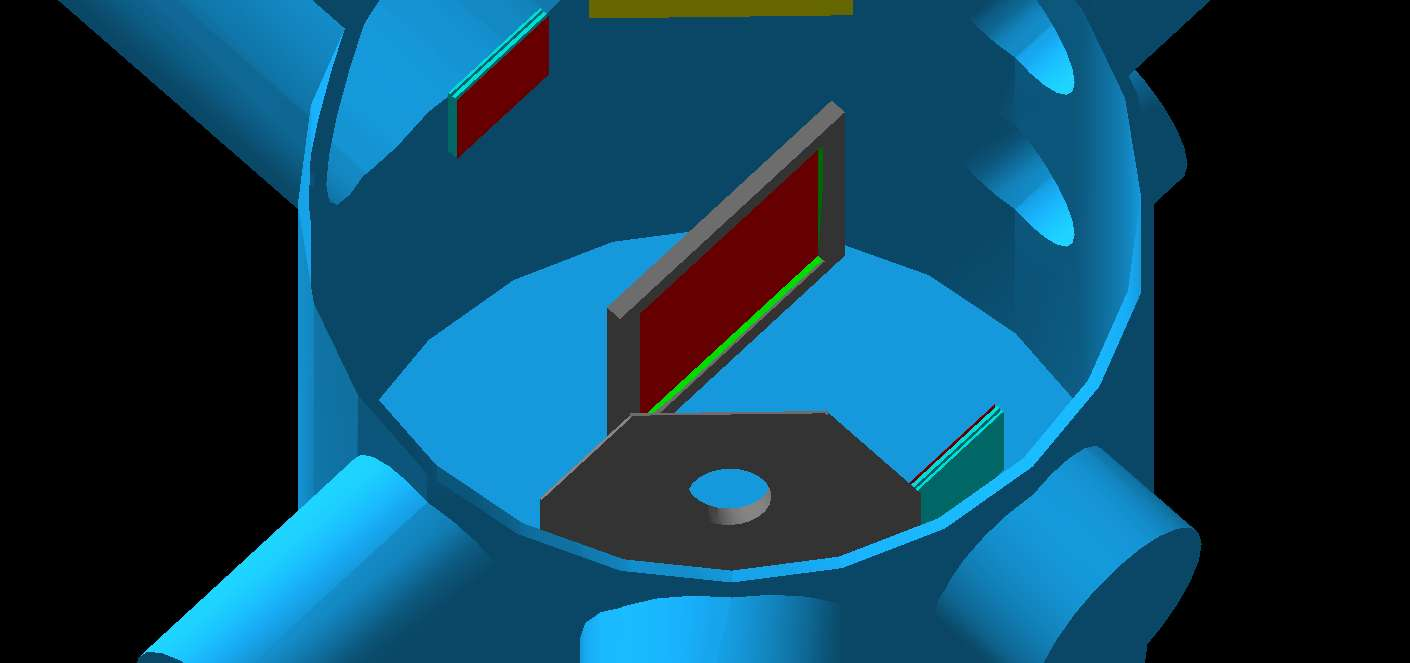
\includegraphics[scale=0.15]{chamber_orientations_pics/chamber_45135_BCout}
    \caption{The beam counter is outside the chamber. The beam left silicon detectors
    are are at a $45^{\circ}$ angle to the beam direction, and the beam right
    silicon detectors are at $135^{\circ}$.}
    \label{fig:chamb_45135_bcout}
  \end{subfigure}
  ~
  \begin{subfigure}[t]{0.45\textwidth}
    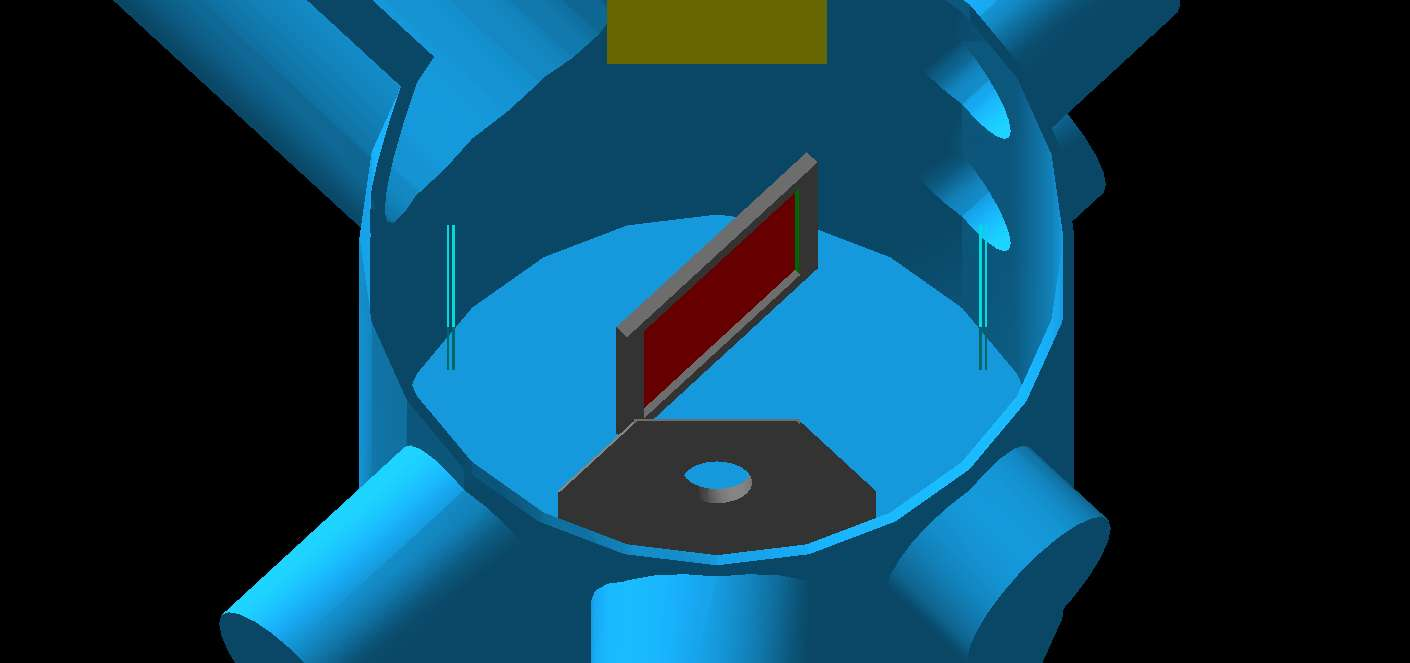
\includegraphics[scale=0.15]{chamber_orientations_pics/chamber_9090_BCout}
    \caption{The beam counter is outside of the chamber, with the beam left and beam
    right silicon detectors both at $90^{\circ}$ to the beam direction.}
    \label{fig:chamb_9090_bcout}
  \end{subfigure}

  \begin{subfigure}[t]{0.45\textwidth}
    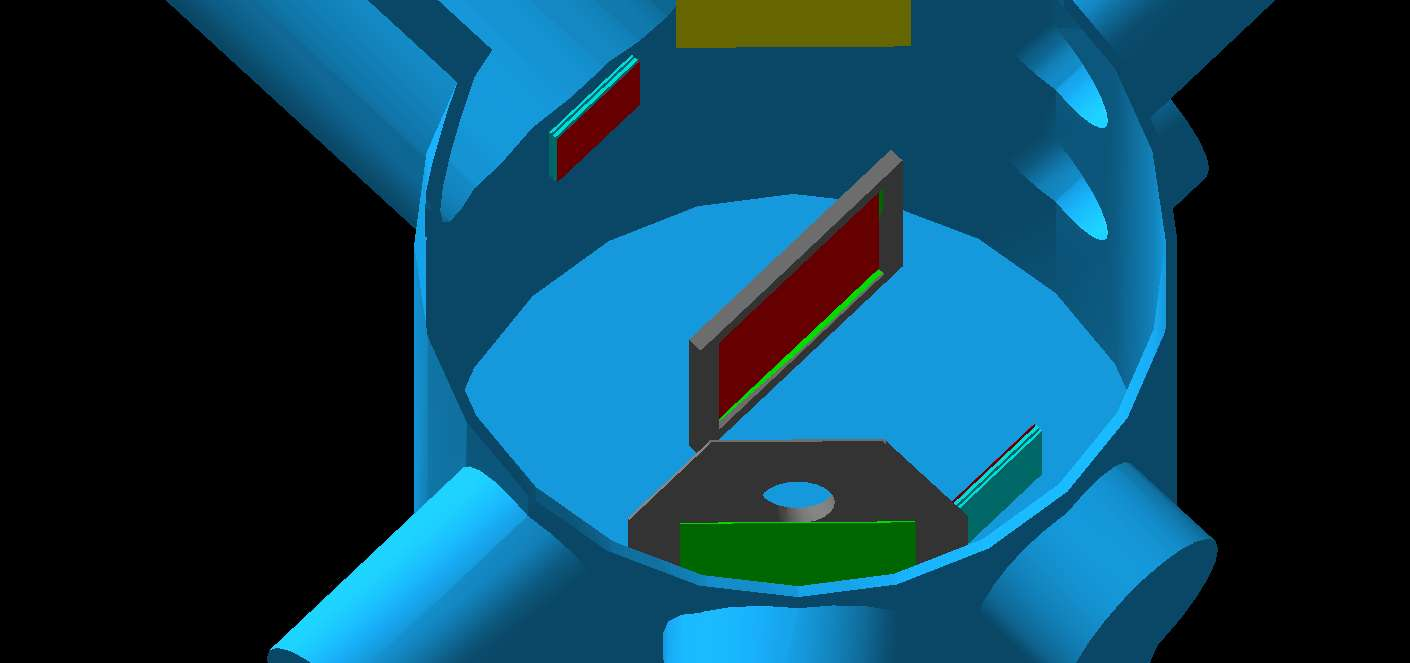
\includegraphics[scale=0.15]{chamber_orientations_pics/chamber_45135_BCin}
    \caption{The beam counter is now inside the chamber, and the silicon detectors
    are back in the $45^{\circ}/135^{\circ}$ orientation.}
    \label{fig:chamb_45135_bcin}
  \end{subfigure}
  ~
  \begin{subfigure}[t]{0.45\textwidth}
    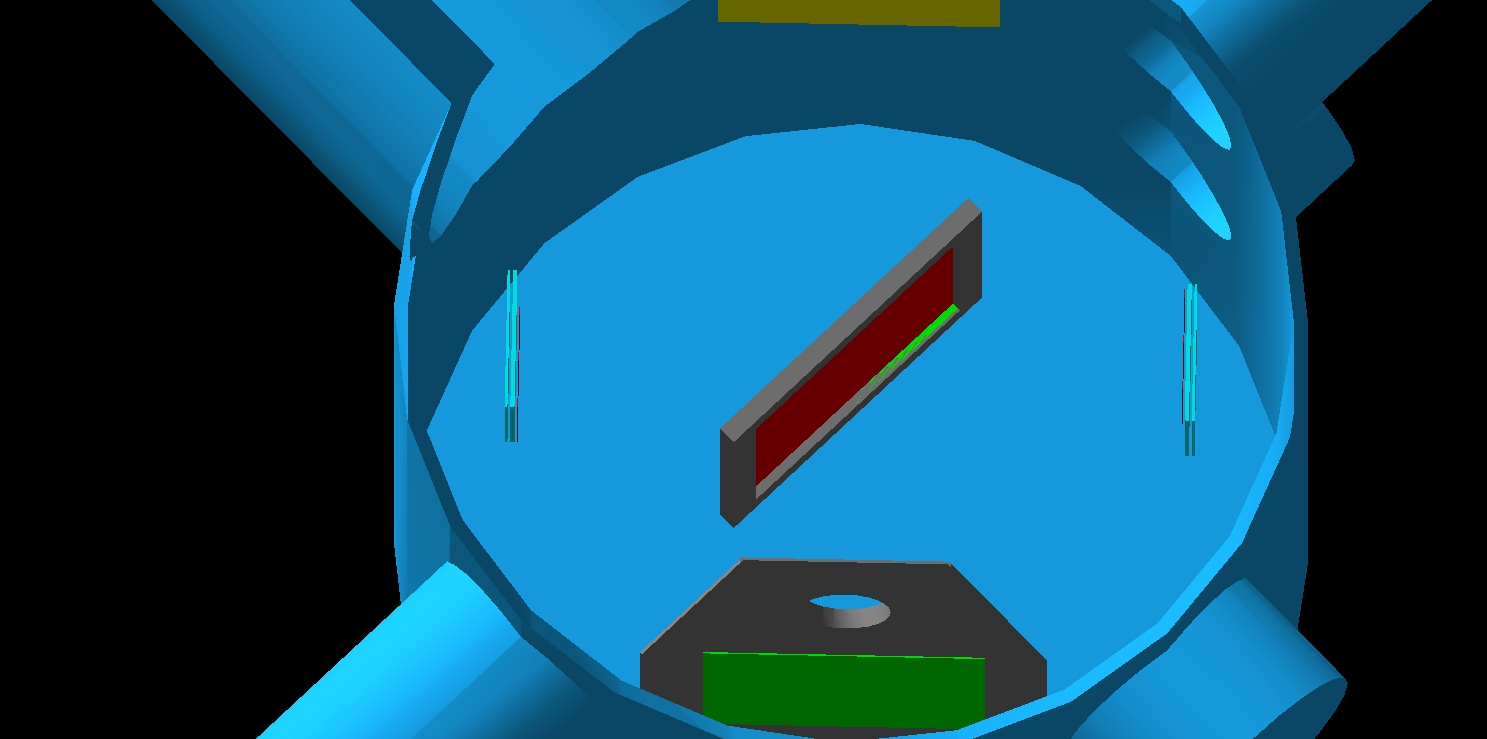
\includegraphics[scale=0.135]{chamber_orientations_pics/chamber_9090_BCin}
    \caption{The beam counter is inside the chamber, and the silicon detector orientation
    is $90^{\circ}/90^{\circ}$.}
    \label{fig:chamb_9090_bcin}
  \end{subfigure}
  \caption{The different chamber geometries. For now we'll mainly stick
  to the top two (with the beam counter, MuSC, outside the chamber).}
  \label{fig:chamb_geos}
\end{figure}

\section{Different Geometries}
There are four major geomitries we will be checking,
seen in Figures \ref{fig:chamb_45135_bcout}-\ref{fig:chamb_9090_bcin}.
The two big variables are whether or not the silicon detectors are
in a $45^{\circ}/135^{\circ}$. and whether the beam counter is inside or
outside the chamber.

\section{Specifications}

Throughout this document I use the term valid to mean

\begin{itemize}
\item Muon entered beam counter (MuSC)
\item Muon did not enter entrance veto (MuSCA)
\item Muon did not enter downstream scintillator (MuVeto)
\end{itemize}

The specifics of the beam and target are

\begin{itemize}
\item Target Material: Aluminum
\item Target Thickness: 50 $\mu$m
\item Beam Momentum: 28.5 MeV/c
\end{itemize}


\section{Scattered Muons}
The primary motivation for the different geometries
is the effect of muons scattering into the silicon detectors. The
numbers can be seen in Table \ref{tab:mu}.

\begin{table}
  \centering
  \begin{tabular}{ c | c c c c c }
    Orientation & Processed & Valid & Stopped & Scattered & Scattered/Valid \\
    \hline \\
    135$^{\circ}$ Beam Right & $11\times10^6$ & 10,530,474 & 1,628,797 & 63 & $3.87\times10^{-5}$ \\
    45$^{\circ}$ Beam Left & $11\times10^6$ & 10,530,474 & 1,628,797 & 9176 & $563.\times10^{-5}$ \\
    90$^{\circ}$ Beam Right & $14.8\times10^6$ & 13,997,538 & 2,498,510 & 128 & $0.914\times10^{-5}$ \\
    90$^{\circ}$ Beam Left & $14.8\times10^6$ & 13,997,538 & 2,498,510 & 172 & $1.23\times10^{-5}$
  \end{tabular}
  \caption{}
  \label{tab:mu}
\end{table}


\section{Proton Energy}
The proton energy deposited in the silicon detectors changes based on the orientation,
and it can be see in Figure \ref{fig:prot_e}.
Additionally, we hope to measure the full energy of protons produced in the target.
Since this isn't necessarily possible, we at least want to maximize
the fraction of the proton energy we measure. Seen in Figure \ref{fig:prot_e}
is also the fraction of the energy measured in the silicone detectors as a function
of the energy of the initial proton.

\begin{figure}
  \begin{subfigure}[t]{0.45\textwidth}
    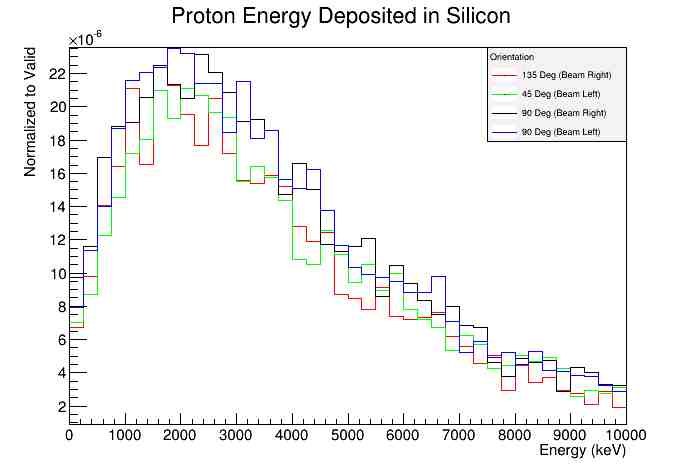
\includegraphics[scale=0.5]{plots/prot_e}
  \end{subfigure}
  
  \begin{subfigure}[t]{0.45\textwidth}
    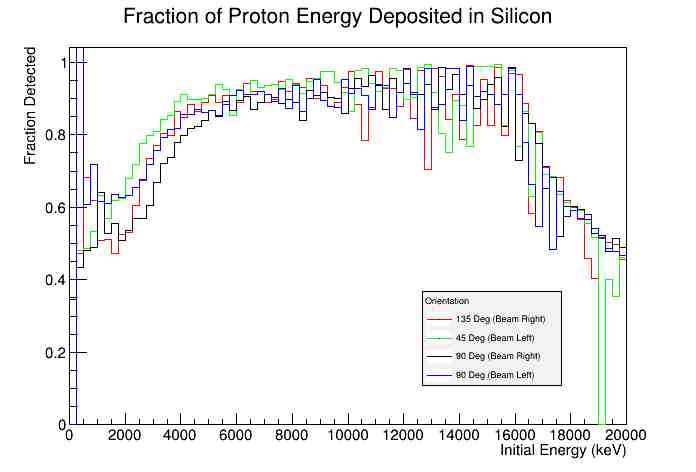
\includegraphics[scale=0.5]{plots/prot_frac}
  \end{subfigure}
  \caption{The energy deposited by the protons in the silicon detectors (top)
    is peaked a little above 2 MeV. The energy fraction (bottom)
    measured drops off at high initial energy (punch-through)
    and low intial energy (large fraction of energy deposited in target).
    There finicky behavior at low energies is a result of protons often not
    escaping the target at low initial energies. Additionally, it seems
    that we do not see a whole lot of punch through until ~15-16 MeV, as
    opposed to the 10 MeV we've been assuming so far.}
  \label{fig:prot_e}
\end{figure}

We can also take a look at the proton transfer functions in Figure \ref{fig:prottrans}.

\begin{figure}
  \centering
  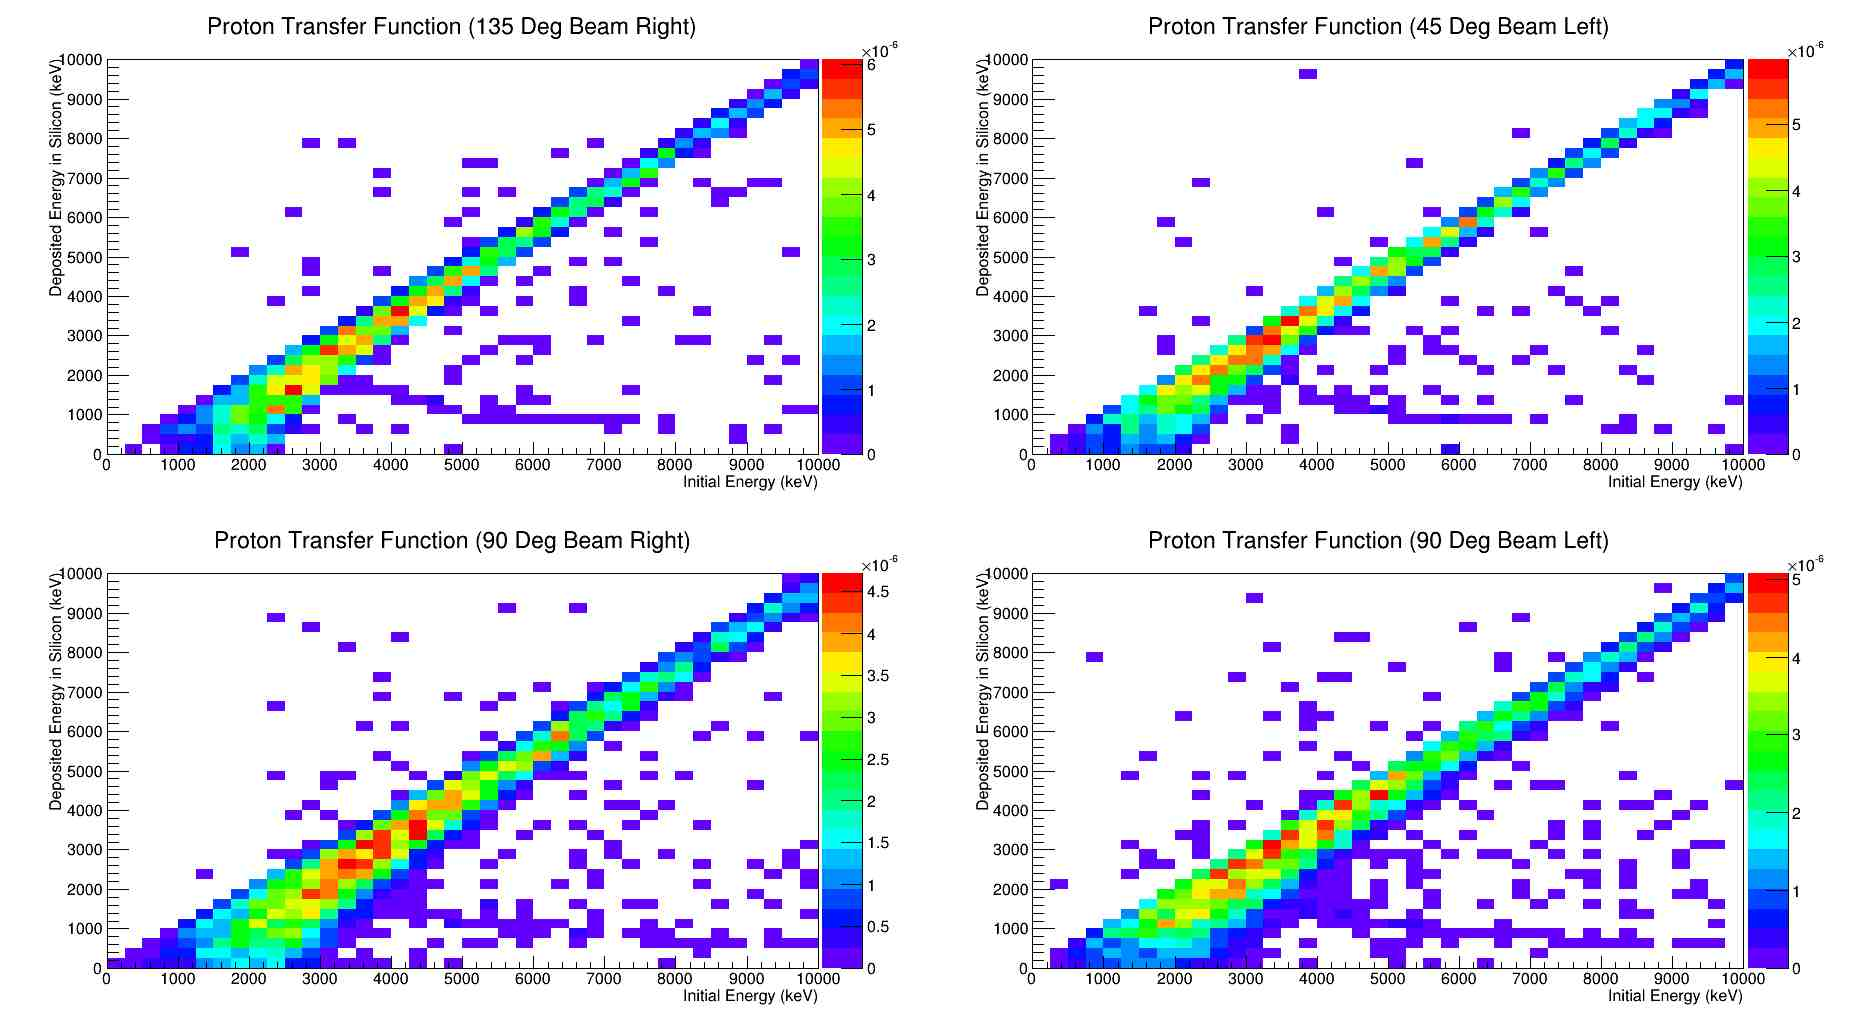
\includegraphics[scale=0.2]{plots/prot_transfunc}
  \caption{Due to the way we count energy, in that once a proton enters the silicon detectors we
    consider \emph{all} energy deposited in those detectors as coming from the proton, we have some
    strange outliers. Otherwise these are in good agreement with \ref{fig:prot_e}.}
  \label{fig:prottrans}
\end{figure}

\section{Electrons After Decay}
Decay in orbit electrons will also be a source of noise. So we can look at
those in Figure \ref{fig:dio_elec}.

\begin{figure}
  \centering
  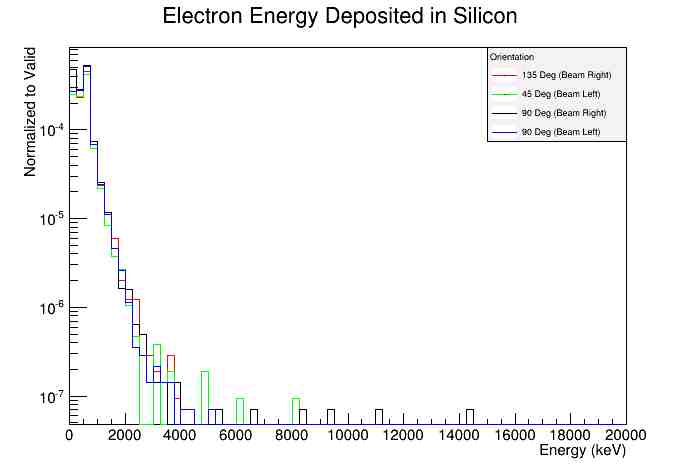
\includegraphics[scale=0.5]{plots/elec_e}
  \caption{The electron energies deposited in the detector arms
    after a decay in orbit occurs in the target. All four orientations are
    shown.}
  \label{fig:dio_elec}
\end{figure}


\section{Source Code}

The cource code has been uploaded to Nam's github, and has several options available in
the input/parameters.txt file. The lengths/thicknesses are apparent (ending in T or L).
The useful options are

\begin{itemize}
\item Deg90:
  True to orient the silicon detectors at 90$^{\circ}$ to the
  beam axis. False for the 45${\circ}$/135${\circ}$ orientation.
\item Target.XX:
  Material to use for the target. True/False for aluminum (XX=Al),
  silicon (XX=Si), and titanium (XX=Ti). If multiple
  are true, then the first that is true in that order is used.
\item Muon:
  True to use muons beam.
\item Electron:
  True to use electron beam. Only checked if Muon is false.
\item Turtle:
  True to use turtle data in input/turtle.root. False to use Gaussian
  parameters set earlier in parameters.txt.
\item MuSCOutside:
  True to have the beam counter outside the chamber, false to have it inside.
\item ProtInTarg:
  Use a histogram of muon stopping locations in the target (input/MuStopDistribution.root)
  to generate protons in the target.
\item Save.Hits:
  True to save vector of TTrackerHits. If not going to be used, can be set to False
  to reduce file size.
\item Save.DR:
  True to save the DetectorResponse vectors. Used in creating pseudo-data and other analysis.
\end{itemize}

\end{document}
